\documentclass{edm_template}

%\usepackage{amsthm,amsmath,amsfonts}
\usepackage{bm}
\usepackage{comment}

\newcommand{\yti}{y_{Ti}}
\newcommand{\yci}{y_{Ci}}
\newcommand{\yhati}{\hat{y}_{Ci}}
\newcommand{\yhat}{\hat{y}_C}
\newcommand{\tauhat}{\hat{\tau}}
\newcommand{\rebar}{\hat{\tau}_{rebar}}
\newcommand{\model}{\hat{y}_0(\cdot)}
\newcommand{\pred}{\hat{y}_0(\bm{x})}
\newcommand{\predi}{\hat{y}_0(\bm{x}_i)}
\newcommand{\EE}{\mathbb{E}}

\newtheorem{prop}{Proposition}


\begin{document}

\title{Using Big Data to Sharpen Design-Based Inference in A/B Tests}

\numberofauthors{4} 
\author{
% 1st. author
\alignauthor Anthony Botelho\\
       \affaddr{Worcester Polytechnic Institute}
       \affaddr{100 Institute Rd}\\
       \affaddr{Worcester, MA 01609}\\
       \email{abotelho@wpi.edu}
% 2nd. author
\alignauthor Adam C Sales\\
       \affaddr{University of Texas at Austin}\\
       \affaddr{536C George I. S\'{a}nchez Building}\\
       \affaddr{Austin, TX 78705}\\
       \email{asales@utexas.edu}
% 3rd. author
\alignauthor Thanaporn Patikorn\\
\affaddr{Worcester Polytechnic Institute}
       \affaddr{100 Institute Rd}\\
       \affaddr{Worcester, MA 01609}\\
       \email{tpatikorn@wpi.edu}
\and  % use '\and' if you need 'another row' of author names
% 4th. author
\alignauthor Neil T. Heffernan\\
\affaddr{Worcester Polytechnic Institute}
       \affaddr{100 Institute Rd}\\
       \affaddr{Worcester, MA 01609}\\
       \email{nth@wpi.edu}
}

\maketitle
\begin{abstract}
Randomized A/B tests in educational software are not run in a vacuum: often, reams of historical data are available alongside the data from a randomized trial. This paper proposes a method to use this historical data--often high-dimensional and longitudinal--to improve causal estimates from A/B tests. The method proceeds in two steps: first, fit a machine learning model to the historical data predicting students' outcomes as a function of their covariates. Then, use that model to predict the outcomes of the randomized students in the A/B test. Finally, use design-based methods to estimate the treatment effect in the A/B test, using prediction errors in place of outcomes. This method retains all of the advantages of design-based inference, while, under certain conditions, yielding more precise estimators. This paper will give a theoretical condition under which the method improves precision, and demonstrates it using a deep learning algorithm to help estimate effects in a set of experiments run inside ASSISTments.
\end{abstract}

\section{Introduction}
(Adam)

\section{Data: 22 Experiments and More}
(March and Anthony)

\section{Rebar}
\subsection{Experiments and Modeling}
To learn if an intervention worked, or to figure out which of two conditions (say, condition 0 and condition 1) produces better outcomes, statistical models can often be quite helpful. 
To take a common example, analysts might regress an outcome $Y$ on an indicator for condition $Z$, along with a vector of covariates $\bm{x}$.
Then, the estimated coefficient on $Z$ is taken as the estimated effect of condition 1 versus 0, controlling for $\bm{x}$. 
The shortcomings of this approach are well-known: if the vector $\bm{x}$ is missing a confounder---a covariate that predicts both subjects' choice of condition, 0 or 1, and outcomes $Y$---then the regression estimate will be biased. 
Moreover, even if there are no unmeasured confounders, if the regression model is misspecified, for instance, modeling the relationship between $Y$ and $\bm{x}$ as linear, then the estimate will also be biased. 
On the other hand, a regression model may be run on all available data, producing precise (if inaccurate) estimates. 

Randomized experiments correct regression's faults. 
If subjects are randomly assigned to conditions 0 or 1, then the difference in mean outcomes between the two groups is an unbiased estimate of the average treatment effect.
More precisely, let $y_{1i}$ be the outcome a subject $i$ \emph{would} experience \emph{if} assigned to condition 1, and let $y_{0i}$ be the outcome $i$ would experience under condition 0.
Then $\bar{y}_1$ is the average outcome that would have occurred had everyone in the experiment been assigned to 1, and $\bar{y}_0$ is the average outcome had everyone been assigned to 0; Their difference, $\bar{y}_1-\bar{y}_0$, is the ``sample average treatment effect,'' or ATE.
A subject's observed outcome $Y_i=\yti$ if $i$ is assigned to 1, $Z_i=1$; $Y_i=\yci$ if $i$ is assigned to 0. 
(Since observed outcomes $Y$ are a function of $Z$, they are random; we may model potential outcomes $y_0$ and $y_1$ as fixed.)
Assuming one subject's assignment to 1 or 0 doesn't affect anyone else's outcome, then $\tauhat\equiv\bar{Y}_{Z=1}-\bar{Y}_{Z=0}$, the difference in mean outcomes between subjects \emph{actually} assigned to 1, and subjects \emph{actually} assigned to 0, is an unbiased estimate of the ATE.
Since $Z$ is randomized, there are no confounders. 
Since the probability distribution of $Z$ is known exactly, no statistical models, or modeling assumptions, are necessary---the analysis may be ``design-based'' instead of model-based.  
On the other hand, any data from the ``remnant'' of an experiment---the set of subjects outside the experiment, who were not randomized to either condition---must be dropped from the analysis. 
Since subjects in the remnant were not randomized, there is no telling how they may differ from the $Z=0$ or $Z=1$ groups, in ways measured or unmeasured, and there is no telling (exactly, statistically) how their data came to be, so design-based analysis is impossible and any model fit to the remnant is most likely misspecified. 
However, though dropping the remnant from the analysis brings unbiasedness, it also brings a loss of precision---all that sample size, thrown away. 

\subsection{A Role for the Remnant} 
Assume the following setup:
a set of users, ``the experimental set'' were randomized to either condition 0 or condition 1, and their outcomes $\bm{Y}$ were measured at the end of the experiment.
The goal of the experiment is to estimate the ATE, $\bar{y}_1-\bar{y}_0$, the average effect in the experimental set. 
Some more subjects, the remnant, were not randomized; instead, they all received condition 0, the default (this isn't strictly necessary---the theory also works if they received condition 1, a mix of conditions, or something else altogether---but it makes things simpler). 
Outcomes $Y$ were also measured for members of the remnant.
Finally, a set of covariates $\bm{x}$, possibly high-dimensional, of mixed-types, and/or longitudinal, were measured for everyone, in the experimental set and in the remnant. 

Experimental estimates typically drop the remnant, and pay the price of lower precision. 
Instead, we suggest training a machine-learning model on the remnant, and using it to ``residualize" the data from the experimental set; we call this algorithm ``remnant-based residualization'' or ``rebar.''
The process is as follows:
\begin{enumerate}
 \item Using data from the remnant, train a model $\model$ to predict $y_0$ as a function of $\bm{x}$.
 \item Validate $\model$ (using cross-validation or other techniques). if it performs well, proceed; otherwise return to step 1, choosing a different model.
 \item Use $\model$ and covariates $\bm{x}$ in the experimental set to generate predicted outcomes $\pred$ and residuals, $e=Y-\pred$.
 \item Estimate the ATE as a difference in mean residuals, $\rebar=\bar{e}_{Z=1}-\bar{e}_{Z=0}$
\end{enumerate}
Just like the traditional estimator $\tauhat$, the rebar estimator $\rebar$ is design-based---its logical basis is the designed experiment, not a model. 
On the other hand, it harvests information from the remnant to improve upon $\tauhat$.

Rebar works because the predictions $\pred$ were generated from an external sample---the remnant---and pre-treatment covariates $\bm{x}$.
Subject $i$'s prediction $\predi$ will be the same whether $i$ is assigned to 0 or to 1---there's no treatment effect on $\pred$.
When treatment is randomized, $Z$ is independent of $\pred$, so, in expectation, the mean of $\pred$ will be equal across the two treatment groups.
  In fact, the rebar estimator can be re-written as $\rebar=\bar{Y}_{Z=1}-\bar{Y}_{Z=0}-(\overline{\pred}_{Z=1}-\overline{\pred}_{Z=0})$. 
The first term is $\tauhat$, which is unbiased for the ATE. The second term is the difference in means of $\pred$, which is zero in expectation---therefore, $\rebar$ is unbiased. 

Rebar's main tool is the model $\model$, which predicts $y_C$ as a function of $\bm{x}$. 
In EDM settings, the dimension of available covariates is very large, and sample sizes are often large as well---machine learning algorithms make strong candidates for $\model$.
$\model$ is not a statistical model \emph{per se}, estimating the parameters of a probability distribution, but as a tool for prediction.
Indeed, it need not be correct in any sense, and its estimates need not be unbiased or consistent. 
Since it is fit on a separate sample from the experimental subjects, the process of fitting it---steps 1 and 2 above---do not affect standard errors, and model misspecification does not lead to bias.

On the other hand, for rebar to be more precise than the usual difference in means, $\model$ must be able to generate decent predictions of $y_C$ in the experimental set. 
This will be the case if $\model{\bm{X}}$ is a good prediction of $y_C$---by residualizing, we subtract out the component of $Y$'s variance that is predicted by $\model{\bm{x}}$. 
In fact, it can be shown that typically, the variance of the rebar estimator is roughly proportionate to the mean-squared prediction error of $\model$ (or, equivalently, the prediction $R^2$) in the experimental set. 


The previous discussion assumed simple randomization. 
However, rebar easily extends to more complex designs.
Further, as we will illustrate below, rebar can be extended to regression estimators of causal effects as well, modeling low-dimensional covariates within sample and high-dimensional covariates out of sample. 


\section{Deep Learning to Predict Completion}
(Anthony)

\section{Results}

\begin{figure}
\centering
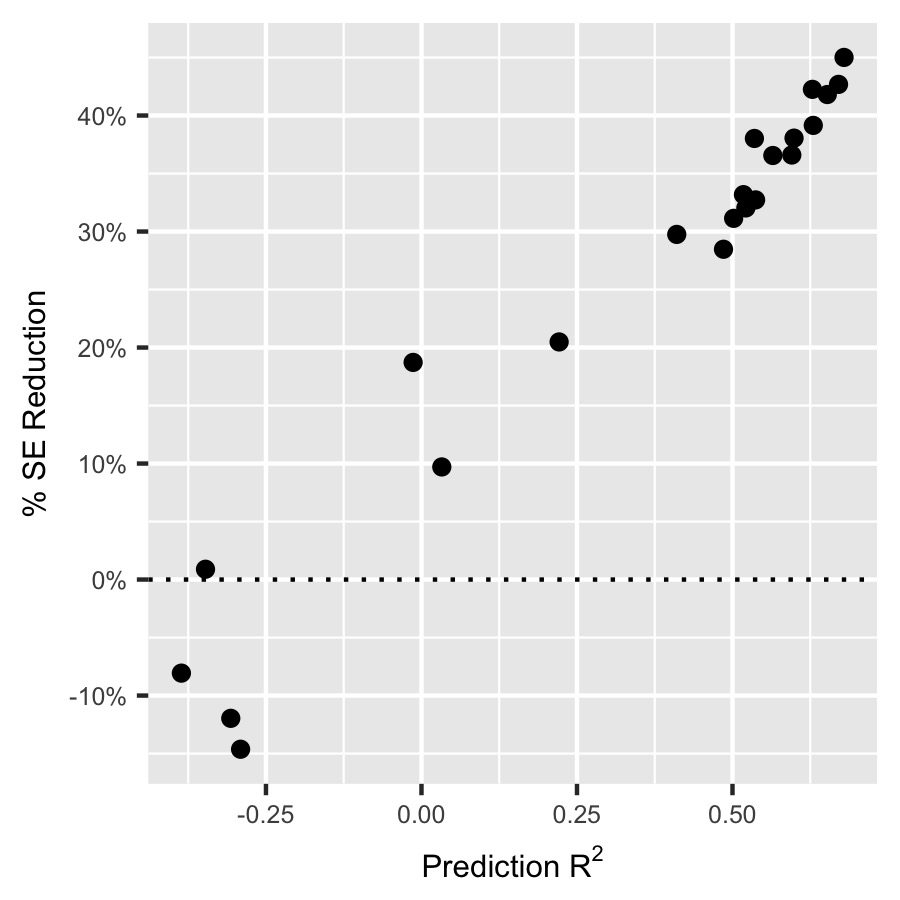
\includegraphics[width=0.5\textwidth]{corVsSE.jpg}
\caption{The improvement in precision of effect estimates as a percentage of the usual precision estimate, $[SE(\tauhat)-SE(\rebar)]/SE(\tauhat)$, plotted as a function of $\model$'s prediction $R^2$ in the experimental set.}
\label{fig:r2se}
\end{figure}

We estimated treatment effects of interventions on skill-builder completion for the 22 experiments using both raw outcomes $\bm{Y}$, the usual approach, and using $\bm{e}=\bm{Y}-\bm{\pred}$, the rebar estimator. 
We also estimated standard errors in both cases.
We used difference in means estimators, so the effect estimates are in units of percentage points---how much more likely were students to finish skill builders under the treatment condition than under control. 

Figure \ref{fig:r2se} shows improvement in precision of the rebar estimator over the usual estimator: the difference of the two standard errors, divided by the usual standard error, $(SE_{usual}-SE_{rebar})/SE_{usual}$.
The x-axis shows the prediction $R^2=1-||Y-\pred||^2/||Y-\bar{Y}||^2$ of the deep learning model when extrapolated to each of the 22 experimental datasets. 
In 19 of the datasets, the rebar standard errors were lower than the usual standard errors. 
In 15 of those datasets, there was a greater than 25\% improvement, and in four datasets the improvement was greater than 40\%.
The extent of the reduction in standard error corresponded closely to the prediction $R^2$ of $\model$, with the most dramatic improvements occurring when $R^2\gtrsim 0.5$.

\begin{figure}
\centering
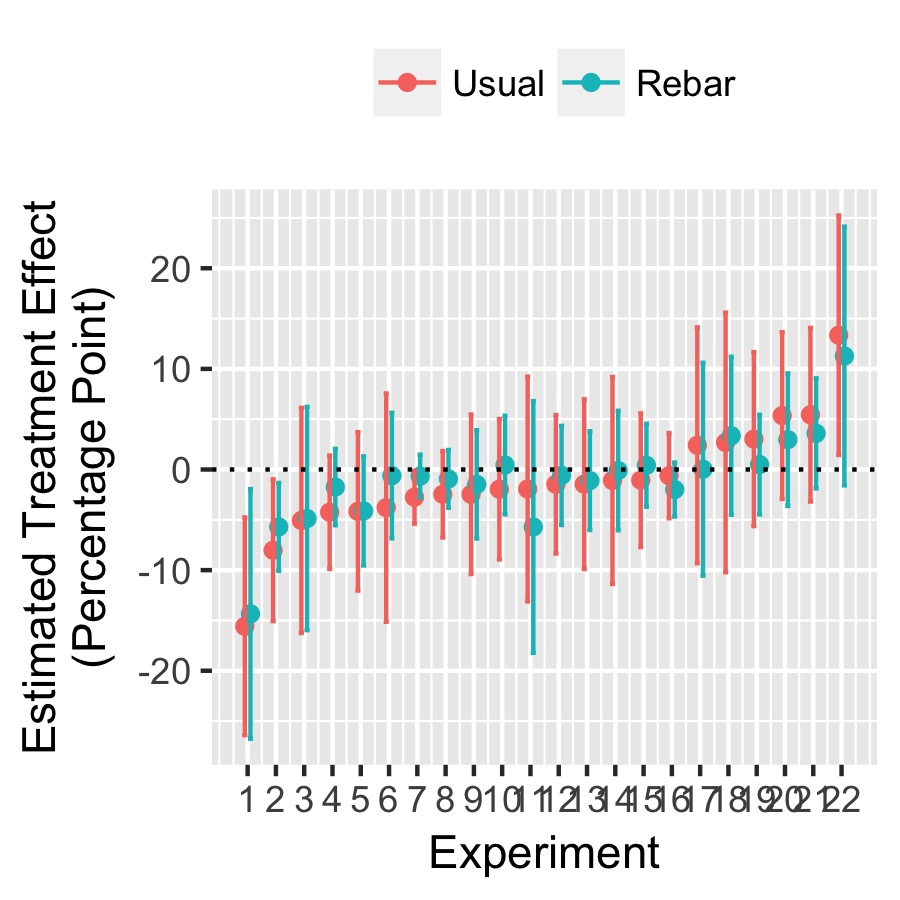
\includegraphics[width=0.5\textwidth]{estEff1.jpg}
\caption{Effect estimates and 95\% confidence intervals for the 22 experiments, using both the usual and rebar estimates. Experiments are ordered by their estimated effect.}
\label{fig:estEff1}
\end{figure}


Figure \ref{fig:estEff1} shows the estimated treatment effects and approximate 95\% confidence intervals (two standard errors in each direction) for the two sets of estimators. 
In all but three cases, the rebar estimate was slightly closer to zero than the usual estimate.
This is what we would expect if most of the true effects were null, so that reducing the noise of the treatment effect estimates would draw them closer to their true values. 
For that reason, although rebar reduced the standard errors in almost all of the experiments, it did not cause any of the non-significant results to become statistically significant. 
In fact, in two cases it had the opposite effect; though this may be disappointing for researchers, it is probably more accurate. 

We also used linear regression to estimate treatment effects, regressing either indicators for completion or prediction errors on indicators for treatment assignment and two covariates: the proportions of students' prior skill builders completed and the proportions of prior skill builder problems students worked that they answered correctly. 
The results, available upon request, are nearly identical.
Although the two covariates improved precision slightly, rebar continued to dominate the usual estimate. 

\begin{comment}
\subsection{Incorporating Regression Controls}
\begin{figure}
\centering
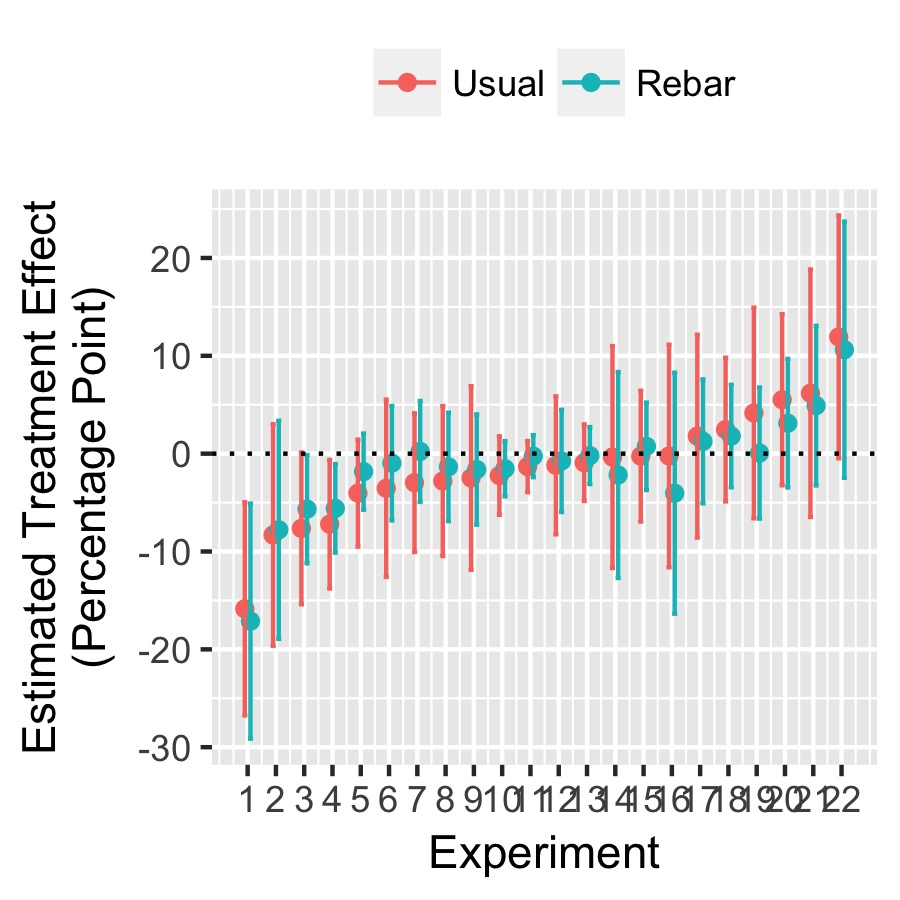
\includegraphics[width=0.5\textwidth]{estEff2.jpg}
\caption{Effect estimates and 95\% confidence intervals for the 22 experiments, from regressions of $Y$ (usual) or $e$ (rebar) on $Z$, prior \% Completed and Prior \% Correct.}
\label{fig:estEff1}
\end{figure}

\begin{figure}
\centering
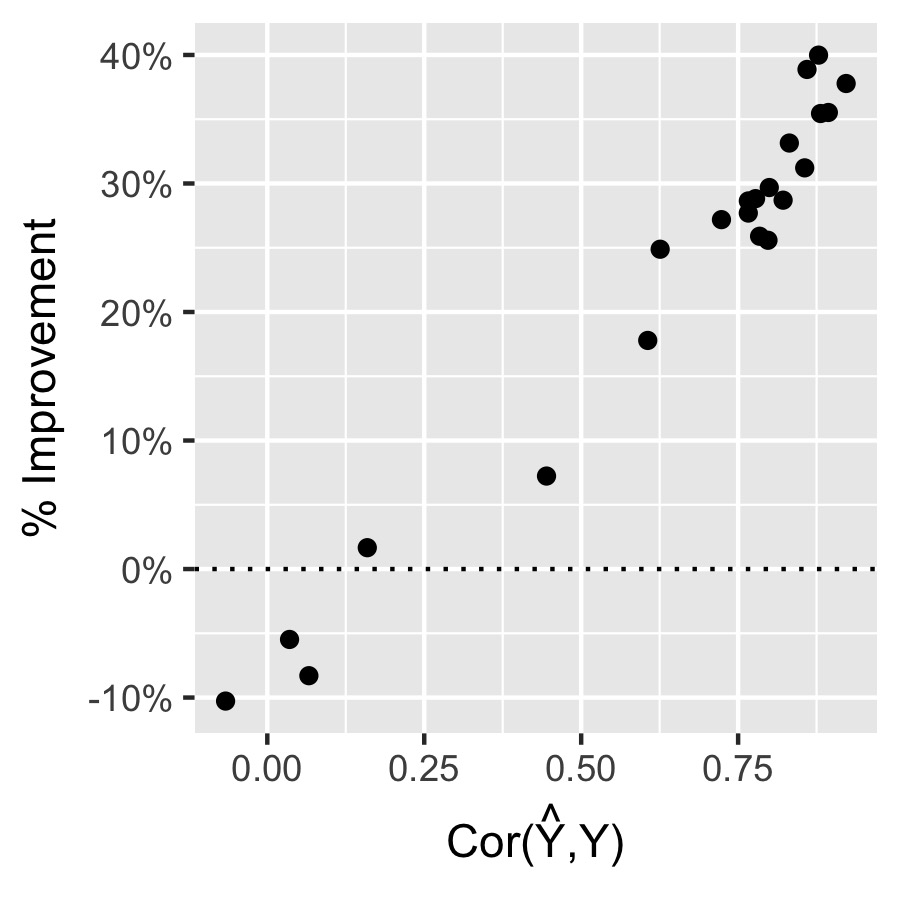
\includegraphics[width=0.5\textwidth]{corVsSE2.jpg}
\caption{The improvement in precision of effect estimates, as a percentage of the usual precision estimate for the usual and rebar regression estimators, plotted as a function of the correlation of outcomes and predictions, $cor(Y,\model{\bm{x}})$.}
\end{figure}
\end{comment}




\section{Discussion}
(Adam)

\bibliographystyle{abbrv}
\bibliography{citations}  
\end{document}
